\let\negmedspace\undefined
\let\negthickspace\undefined
\documentclass[journal]{IEEEtran}
\usepackage[a5paper, margin=10mm, onecolumn]{geometry}
%\usepackage{lmodern} % Ensure lmodern is loaded for pdflatex
% \usepackage{tfrupee} % Include tfrupee package

\setlength{\headheight}{1cm} % Set the height of the header box
\setlength{\headsep}{0mm}     % Set the distance between the header box and the top of the text

\usepackage{gvv-book}
\usepackage{gvv}
\usepackage{cite}
\usepackage{amsmath,amssymb,amsfonts,amsthm}
\usepackage{algorithm}
\usepackage{algorithmic}
\usepackage{graphicx}
\usepackage{textcomp}
\usepackage{xcolor}
\usepackage{txfonts}
\usepackage{listings}
\usepackage{enumitem}
\usepackage{mathtools}
\usepackage{gensymb}
\usepackage{comment}
\usepackage[breaklinks=true]{hyperref}
\usepackage{tkz-euclide} 
\usepackage{listings}
% \usepackage{gvv}                                        
\def\inputGnumericTable{}                                 
\usepackage[latin1]{inputenc}                                
\usepackage{color}                                            
\usepackage{array}                                            
\usepackage{longtable}                                       
\usepackage{calc}                                             
\usepackage{multirow}                                         
\usepackage{hhline}                                           
\usepackage{ifthen}                                           
\usepackage{lscape}
% \usepackage{algpseudocode}
\begin{document}

\bibliographystyle{IEEEtran}
\vspace{3cm}

\title{NCERT 9.5.1}
\author{EE24BTECH11053 - S A Aravind Eswar}
% \maketitle
% \newpage
% \bigskip
{\let\newpage\relax\maketitle}

\renewcommand{\thefigure}{\theenumi}
\renewcommand{\thetable}{\theenumi}
\setlength{\intextsep}{10pt} % Space between text and floats

\textbf{Question:} Solve the differential equation given below with initial conditions $ x = 0 $ and $ y = 0 $.
\begin{align}
	\frac{dy}{dx} + 2y = \sin{x}
\end{align}
\subsection{Theoretical Solution}
% \begin{enumerate}
    % \item We can realise that the given equation is a linear differential equation. Then,
    % \begin{align}
	%     P &= 2\\
    %     Q &= \sin{x}
    % \end{align}

    % \item Multiplying on both sides with $e^{\int P}$ which is, $e^{2x}$

    % \begin{align}
	%     e^{2x}\, \frac{dy}{dx} + 2e^{2x} y = \sin{x}\, e^{2x}
    % \end{align}
    
    % \item This can be written as,
    % \begin{align}
	%     \frac{d}{dx}\brak{y\, e^{2x}} = \sin{x}\, e^{2x}
    % \end{align}

    % \item Integrating on both sides with respect to $dx$, we get,

    % \begin{align}
	%     y\, e^{2x} = e^{2x}\, \frac{2\sin{x} - \cos{x}}{5} + C
    % \end{align}

    % \item Diving on both sides with $e^{2x}$ we get,

    % \begin{align}
	%     y = \frac{2 \sin{x} - \cos{x} + C\, e^{-2x}}{5}
    % \end{align}

    
    % \item Applying the inital conditions $x = 0$ and $y = 0$, we get,

    % \begin{align}
    %     C = 1
    % \end{align}

    % \item Thus,

    % \begin{align}
    %     y &= \frac{2 \sin{x} - \cos{x} + \, e^{-2x}}{5}
    % \end{align}
    % is the solution of the given differential equation with given inital conditions\\
    
    The Given equation can be written as,
    \begin{align}
        y^\prime + 2y = \sin{x}
    \end{align}

    Applying Laplace Transform on both sides,

    \begin{align}
        \mathcal{L}{\cbrak{y^\prime}} + 2\mathcal{L}\cbrak{y} = \mathcal{L}\cbrak{\sin{x}}\\
        \cbrak{s\,Y - y(0)} + 2\cbrak{Y} = \frac{1}{s^2 + 1}
    \end{align}

    This can be reduced to the following form, and applying the inital condition,

    \begin{align}
        Y = \frac{1}{(s+2)(s^2+1)}
    \end{align}

    Decomposing the partial fraction,

    \begin{align}
        Y = \brak{\frac{2}{s^2 + 1} - \frac{s}{s^2 + 1} + \frac{1}{s+2}}\frac{1}{5}
    \end{align}

    Now, applying inverse transform, we get the solution,

    \begin{align}
        y = \frac{2\sin{x}-\cos{x}+e^{-2x}}{5}
    \end{align}

    \subsection{Finite Differences}
       The Difference Equation is given by,
       \begin{align}
        \frac{dy}{dx} \approx \frac{y_{n+1} - y_n}{h}
       \end{align}

       This can be written as,
       \begin{align}
            y_{n+1} = y_n + \frac{dy}{dx} \, h
       \end{align}

       Given that,
       \begin{align}
        \frac{dy}{dx} = \sin{x} - 2y
       \end{align}

       The Difference equation can be written as,
       \begin{align}
        y_{n+1} = y_n + \brak{\sin{x_n} - 2y_n}\, h
       \end{align}

    % This can be implemented as an algorithm as following,

    
    % \begin{algorithm}[!h]
    %     \caption{Finite Difference Algorithm}
    %     \begin{algorithmic}
    %         \STATE \text{Initial condition, } $x_0 \gets 0$\\
    %         % \STATE \text{End value of domain, } $x_2 \gets 5$\\
    %         % \STATE $x \gets$ linspace($x_1$, $x_2$, $resolution$)
    %         % \STATE $y \gets$ array of size($resolution$)
    %         \STATE $y_0 \gets 0$
    %         \STATE \text{Number of iterations, } $iterations \gets 20$\\
    %         \STATE \text{Step size, } $h = 0.25$
    %         \FOR{$i$ in range(1, $iterations$)}
    %             \STATE $\displaystyle y_{i} = y_{i-1} + \brak{\sin{x_{i-1}} - 2y_{i-1}}\, h$
    %             \STATE $x_i \gets x_{i-1} + h$
    %         \ENDFOR
    %         \STATE plot($x, y$)
    %     \end{algorithmic}
    % \end{algorithm}
    % \newpage
    Below is verification:
    \begin{figure}[ht]  
        \centering  
        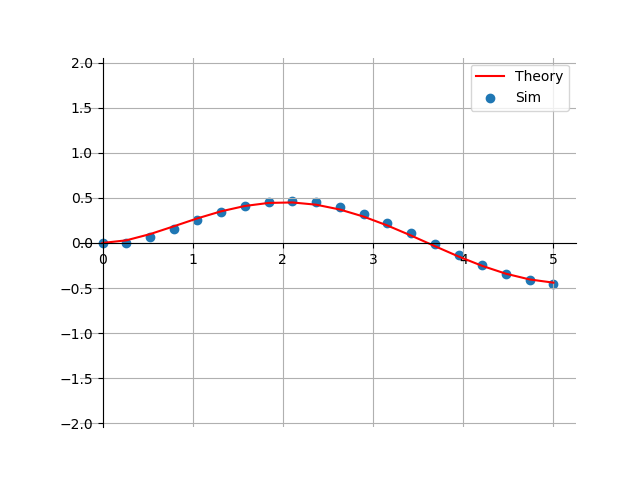
\includegraphics[width=\columnwidth]{figs/fig1_.png}  
        \caption{Verification}
        % \columnwidth
    \end{figure}


% \end{enumerate}

\end{document}